\documentclass{report}
\usepackage[italian]{babel}
\usepackage[hidelinks]{hyperref}
\usepackage{graphicx}
\usepackage{algorithm}
\usepackage{capt-of}
\usepackage{amsmath}
\usepackage{longtable}
\usepackage{caption}
\usepackage{booktabs}
\usepackage{algpseudocode}
\usepackage{makecell}
\usepackage[utf8]{inputenc}
\usepackage{fixltx2e}
\usepackage{listings}
\usepackage{lipsum}% http://ctan.org/pkg/lipsum
\author{Alberto Bezzon, Tommaso Carraro, Matteo Ceradini} \title{Combinare sistemi di reputazione e di raccomandazione per ottenere consigli migliori online} \date{\today}
\setcounter{tocdepth}{6}
\setcounter{secnumdepth}{6}
\renewcommand{\thesection}{\arabic{section}}%
\newcommand{\myparagraph}[1]{\paragraph{#1}\mbox{} \mbox{}}
\begin{document}
	\maketitle
	\tableofcontents
	\listoffigures
	\listoftables
	\newpage
	\renewcommand*{\arraystretch}{2}
	\hypertarget{header-n0}{%
		\section{Introduzione}\label{header-n0}}
	
	\hypertarget{header-n2}{%
		\subsection{Sistemi di raccomandazione}\label{header-n2}}
	
	Su Internet la quantità di informazioni è travolgente e continuamente in
	aumento, questo ha reso impossibile l'accesso tempestivo a elementi e
	informazioni di interesse sulla rete. I sistemi di recupero delle
	informazioni (ad esempio i motori di ricerca) hanno parzialmente risolto
	il problema ma priorità e personalizzazione (mappare i contenuti
	disponibili per gli interessi e le preferenze dell'utente) di
	informazioni erano assenti. Per tale motivo sono stati introdotti i sistemi di raccomandazione.
	
	I \emph{Sistemi di Raccomandazione} sono sistemi di filtraggio di
	informazioni correlate alle preferenze dell'utente, all'interesse o al
	comportamento osservato su di esso rispetto alla grande quantità di
	informazioni. Questi sistemi hanno la capacità di prevedere se un
	determinato utente preferirebbe un articolo o meno in base al profilo
	dell'utente.
	
	I sistemi di raccomandazione portano dei vantaggi sia agli utenti,
	mostrando informazioni di interesse, sia per i fornitori di servizi
	perché riducono i costi di transazione per la ricerca e la selezione di
	articoli in ambiente di shopping online. Essi migliorano le entrate in
	quanto sono mezzi efficaci per vendere più prodotti.
	
	Lo scopo dei sistemi di raccomandazione è principalmente di generare
	suggerimenti su risorse di cui un utente, a priori non ne è a conoscenza
	ma probabilmente potrebbe essere interessato ad esse.
	
	\hypertarget{header-n15}{%
		\subsection{Sistemi di reputazione}\label{header-n15}}
	
	I \emph{Sistemi di Reputazione} sono un componente essenziale di varie
	piattaforme online, come ad esempio siti di e-commerce o sistemi di
	condivisione di file. Questi sistemi incoraggiano gli utenti a fornire
	un feedback su esperienze passate. Nascono perché, prima di essi, gli
	utenti che interagivano con nuovi siti web non avevano alcuna
	informazione.
	
	Lo scopo dei sistemi di reputazione è quello di fornire consigli su
	risorse di cui l'utente è interessato e di cui ne è già a conoscenza.
	
	\hypertarget{header-n20}{%
		\subsection{Combinazione tra sistemi di raccomandazione e sistemi di
			reputazione}\label{header-n20}}
	
	I sistemi di reputazione e raccomandazione
	sono basati su principi differenti ma hanno entrambi lo stesso scopo:
	supportare l'utente fornendo delle informazioni per agevolare le sue
	decisioni. Brevemente, i compiti dei due sistemi sono i seguenti:
	
	\begin{itemize}
		\item
		sistemi di raccomandazione: suggeriscono all'utente risorse che non
		conosce ma alle quali può essere interessato. I valori di
		raccomandazione sono calcolati basandosi su informazioni fornite da
		altri utenti per oggetti simili;
		\item
		sistemi di reputazione: forniscono alla comunità informazioni
		riguardanti risorse che l'utente conosce già. I punteggi di
		reputazione indicano quanto un oggetto è piaciuto ad un utente.
	\end{itemize}
	
	Per fornire delle raccomandazioni più accurate è possibile integrare i
	due sistemi. L'integrazione risulta complessa a causa della diversità
	dei sistemi che hanno forme diverse di feedback. Anche i risultati hanno
	forme diverse:
	
	\begin{itemize}
		\item
		un voto da 1 a 5 per i sistemi di reputazione;
		\item
		una tupla $(d\textsubscript{1}, ... , d\textsubscript{k})$, dove $d_i$ è una diversa caratteristica della
		risorsa $d$, per i sistemi di raccomandazione.
	\end{itemize}
	
	Nella sezione §2 viene riassunta una soluzione analizzata e studiata.
	Nella sezione §3 viene presentata una soluzione che utilizza i vincoli
	soft.
	\newpage
	\hypertarget{header-n25}{%
		\section{Soluzione di Josang e co.}\label{header-n25}}
	
	\hypertarget{header-n26}{%
		\subsection{Introduzione}\label{header-n26}}
	
	La soluzione del Professor Josang e dei suoi colleghi consiste nel
	fondere i punteggi di reputazione e di raccomandazione tramite un
	operatore chiamato CasMin (Cascading Minimum Common Belief Fusion). Il
	problema principale è che i punteggi di reputazione sono potenzialmente
	diversi dai valori di raccomandazione, ossia sono eterogenei e quindi
	impossibili da fondere senza prima essere manipolati. Per applicare
	l'operatore CasMin a tali punteggi bisogna renderli prima di tutto
	omogenei. Per rendere omogenei i punteggi di reputazione e i valori di
	raccomandazione, essi devono essere mappati in opinioni soggettive. Dopo
	essere stati mappati in opinioni soggettive, i punteggi possono essere
	combinati con l'operatore CasMin che restituirà un valore alto solo se
	entrambi i punteggi, di reputazione e di raccomandazione
	rispettivamente, saranno alti. Una risorsa verrà suggerita all'utente
	solo se è stata raccomandata con alta confidenza e se ha un alto
	punteggio di reputazione. La raccomandazione diviene più accurata
	rispetto al solo sistema di raccomandazione che può raccomandare
	oggetti con bassa reputazione. Infine i consigli distribuiti agli utenti
	avranno una qualità migliore.
	
	\hypertarget{header-n47}{%
		\subsection{Opinioni soggettive}\label{header-n47}}
	
	In questa sezione viene introdotta la notazione e la formazione delle
	opinioni soggettive usate per fondere gusto e fiducia. Successivamente
	viene descritto un metodo per mappare dei punteggi multinomiali in
	opinioni binomiali. I punteggi multinomiali sono la forma di feedback più comune
	restituita dai sistemi di reputazione e dai sistemi di raccomandazione.
	
	\hypertarget{header-n50}{%
		\subsubsection{Formazione e rappresentazione}\label{header-n50}}
	
	Un'opinione soggettiva esprime la credenza (belief) degli stati di uno
	spazio degli stati chiamato ``frame". Uno stato in un frame può essere
	considerato come una dichiarazione, quindi un frame contiene un insieme
	di dichiarazioni. Indichiamo con $X = \{x\textsubscript{1}, x\textsubscript{2}, ... , x\textsubscript{k}\}$ un frame di
	cardinalità $k$, dove $x\textsubscript{i} (1\le i \le k)$ rappresenta uno
	specifico stato. Un'opinione distribuisce la massa di credenze sul
	ridotto powerset del frame, indicato con $R(X)$.
	
	Un'opinione è una funzione composta che consiste in un vettore di belief
	\textbf{b}, un parametro di incertezza \textbf{u} e un vettore di base
	rate \textbf{a}, che prende valori nell'intervallo ${[}0,1{]}$ e che
	soddisfa i seguenti requisiti di additività:
	
	\begin{itemize}
		\item
		\textbf{Additività belief}: \begin{equation} u_X +\sum_{x_i \in R(X)}b_X(x_i)=1 \label{equazione1};\end{equation}
		\item
		\textbf{Additività base rate}: \begin{equation}\sum_{i=1}^k a_X(x_i)=1 \textnormal{, dove } x_i \in X \label{equazione2}.\end{equation}
	\end{itemize}
	
	L'opinione di un utente A sul frame $X$ è denotata come $\omega \textsuperscript{A}\textsubscript{X} =
	(b\textsubscript{X},u\textsubscript{X},a\textsubscript{X})$, dove $b\textsubscript{X}$ è un vettore di belief sugli stati di $R(X)$,
	$u\textsubscript{X}$ è la massa di incertezza complementare, e $a\textsubscript{X}$ è un vettore di base
	rate su $X$, tutti visti dal punto di vista del proprietario delle belief
	A.
	
	\hypertarget{header-n64}{%
		\subsubsection{Tipologie di opinioni soggettive}\label{header-n64}}
	
	Vengono presentate due diverse tipologie di opinioni soggettive:
	
	\begin{itemize}
		\item
		Opinioni multinomiali: il vettore di belief $b\textsubscript{X}$ viene
		applicato solamente agli elementi $x\textsubscript{i}$ appartenenti a $X$, e non in $R(X)$;
		\item
		Opinioni binomiali: vengono applicate ai frame binari e hanno una
		rappresentazione speciale. Indichiamo con $X = \{x,\overline{x}\}$ un frame
		binario. Un'opinione binomiale sulla verità dello stato $x$ è la
		quadrupla ordinata $\omega\textsubscript{X}=(b,d,u,a)$, dove:
		
		\begin{itemize}
			\item
			$b$(belief): è la massa di credenze in supporto che $x$ sia vero;
			\item
			$d$(disbelief): è la massa di credenze in supporto che $x$ sia falso;
			\item
			$u$(incertezza): è l'incertezza sulla probabilità di $x$;
			\item
			$a$(base rate): è la probabilità preventiva non informativa di $x$.
		\end{itemize}
	\end{itemize}
	
	In caso di opinioni binomiali l'equazione \eqref{equazione1} è espressa come:
	\begin{center}
	\begin{equation}
	b+d+u=1. \label{equazione3}
	\end{equation}
	
	\end{center}
	
	\hypertarget{header-n89}{%
		\subsubsection{Conversione di opinioni multinomiali in opinioni
			binomiali}\label{header-n89}}
	
	Le opinioni multinomiali sono una generalizzazione delle opinioni
	binomiali e in certi casi può essere necessario proiettare le opinioni
	multinomiali in opinioni binomiali. Per esempio, un sistema di
	reputazione dove i punteggi sono dati nella forma 1-5 stelle può
	rappresentare un punteggio di reputazione come un'opinione multinomiale
	su un frame con 5 stati, ognuno dei quali rappresenta uno specifico
	numero di stelle. In questo caso, un punteggio di reputazione
	rappresentato come un'opinione multinomiale può essere proiettato in
	un'opinione binomiale nel modo seguente.
	
	Indichiamo con $X=\{x\textsubscript{1},...,x\textsubscript{k}\}$ un frame dove i $k$ stati rappresentano un
	livello crescente di punteggio. Indichiamo con $Y=\{y,\overline{y}\}$ un frame
	frame binario dove $y$ e $\overline{y}$ indicano un'alta qualità e una bassa qualità
	di una risorsa, rispettivamente. Assumiamo che un punteggio di
	reputazione o un valore di raccomandazione siano espressi tramite
	l'opinione multinomiale $\omega\textsubscript{X}=(b\textsubscript{X},u\textsubscript{X},a\textsubscript{X})$ sul frame $X$, e che un'opinione
	binomiale $\omega\textsubscript{y}=(b\textsubscript{y},d\textsubscript{y},u\textsubscript{y},a\textsubscript{y})$ è richiesta sul frame binario $Y$. Allora la
	proiezione dall'opinione multinomiale $\omega\textsubscript{X}$ su $X$ nella opinione
	binomiale $\omega\textsubscript{y}$ su $Y$ è definita da: 
	
	\begin{center}
	\begin{equation}
	\begin{cases}
		u_y=u_X\\
		b_y=\sum_{i=1}^k b_{x_i} \frac{(i-1)}{(k-1)}\\
		d_y=1-b_y-u_y\\
		a_y=\sum_{i=1}^k a_{x_i} \frac{(i-1)}{(k-1)}
	\end{cases} \label{equazione4}
	\end{equation}
	\end{center}
	
	
	Il vantaggio di proiettare opinioni multinomiali in opinioni binomiali è
	la flessibilità di analizzare i punteggi di reputazione e i valori di
	raccomandazione indipendentemente dalla cardinalità del frame.
	
	\hypertarget{header-n96}{%
		\subsection{Determinazione delle opinioni}\label{header-n96}}
	
	In questa sezione vengono descritte le procedure per derivare opinioni
	soggettive dai punteggi di reputazione e dai valori di raccomandazione
	prodotti dai sistemi di reputazione e dai sistemi di raccomandazione,
	rispettivamente.
	
	\hypertarget{header-n99}{%
		\subsubsection{Opinioni derivate dai sistemi di
			reputazione}\label{header-n99}}
	
	Un sistema di reputazione generalmente si applica a servizi o beni che
	possono essere valutati su uno o più aspetti. Nel caso in cui solamente
	un singolo aspetto può essere valutato, esso rappresenta tipicamente la
	qualità totale di uno specifico servizio o bene. Ogni aspetto può essere
	valutato con uno specifico livello di qualità, ad esempio da 1 a 5
	stelle. È possibile che per un aspetto possano essere assegnati solo due
	possibili livelli di qualità, ad esempio ``pollice in su" e ``pollice in
	giù". In quest'ultimo caso i livelli indicano una buona qualità o una
	cattiva qualità, rispettivamente.
	
	Le opinioni per ogni aspetto possono essere derivate da tali
	valutazioni. Il frame per ogni aspetto è composto dall'insieme di
	livelli di punteggio discreti che possono essere assegnati all'aspetto,
	quindi nel caso in cui per un aspetto si possa assegnare una valutazione
	da 1 a 5 stelle, il frame corrispondente avrà 5 stati. Indichiamo con $X$
	il frame di cardinalità $k$, con $r(x\textsubscript{i})$ il numero di punteggi assegnati del
	tipo $x\textsubscript{i}$, e con $\omega\textsubscript{X} =(b\textsubscript{X},u,a\textsubscript{X})$ un'opinione multinomiale su $X$. Più punteggi
	vengono raccolti e minore sarà l'incertezza. L'opinione $\omega\textsubscript{X}$ può
	essere determinata dai punteggi $r(x\textsubscript{i})$ tramite la seguente equazione:
	
	\begin{center}
	\begin{equation}
		\forall x_i \in X \begin{cases}
								b(x_i)=\frac{r(x_i)}{W+\sum_{i=1}^k r(x_i)}\\
								u=\frac{W}{W+\sum_{i=1}^k r(x_i)}
							\end{cases}
							\label{equazione5}
	\end{equation}
	\end{center}
	
	
	
	Nell'equazione $W = 2$ è il peso precedente non informativo con valore di
	default imposto dal requisito di avere una funzione di densità di
	probabilità uniforme su frame binari.
	
	Un punteggio è espresso come uno specifico livello corrispondente ad un
	singolo stato nel frame. Nel caso in cui dovessero esserci più di due
	livelli di punteggio, le opinioni derivate saranno multinomiali. Dualmente,
	nel caso in cui solo due tipi di valutazione possono essere dati, il
	frame sarà binario e quindi le opinioni derivate saranno binomiali. I punteggi
	di reputazione espressi come opinioni multinomiali possono essere
	mappati in opinioni binomiali assumendo che ogni livello di punteggio
	corrisponda ad un valore compreso nell'intervallo ${[}0,1{]}$.
	
	\hypertarget{header-n108}{%
		\subsubsection{Opinioni derivate dai sistemi di
			raccomandazione}\label{header-n108}}
	
	Nel nostro progetto i valori di raccomandazione sono generati da un
	metodo CF (Collaborative filtering) basato sull'utente. Il compito dei
	metodi CF è di predire la preferenza di una data risorsa per un utente
	attivo, basandosi sulla storia dell'utente stesso e degli altri
	partecipanti della comunità. Vengono introdotti i simboli $s,v$ per gli
	utenti e $i,j$ per gli oggetti. Indichiamo con $R\textsubscript{v,i}$ il punteggio dato da
	un utente $v$ all'oggetto $i$, e con $I\textsubscript{v}$ l'insieme degli oggetti che l'utente
	$v$ ha precedentemente votato. Il punteggio medio dell'utente $v$ è dato
	dalla seguente formula:
	
	\begin{center}
	\begin{equation}
		\overline{r}_v=\frac{1}{|I_v|} \sum_{i \in Iv} r_{v,i}
		\label{equazione6}
	\end{equation}
	\end{center}
	
	Indichiamo con $N\textsubscript{s,j}$ il vicinato di un utente attivo $s$ vincolato
	dall'aver votato l'oggetto $j$. Quindi $N\textsubscript{s,j}$ è l'insieme di utenti che
	hanno votato gli stessi (o alcuni) oggetti che anche $s$ ha votato e che
	hanno votato anche lo specifico oggetto $j$. Generalmente, solo i migliori
	$K$ utenti più simili a $s$ vengono selezionati per far parte del vicinato.
	La predizione $p\textsubscript{s,j}$ per l'utente $s$ sull'oggetto $j$ è data dalla seguente
	formula:
	
	\begin{center}
		\begin{equation}
			p_{s,j}=\overline{r}_s+k \sum_{v \in N_{s,j}}w(s,v)(r_{v,j}-\overline{r}_v),
			\label{equazione7}
		\end{equation}
		
	\end{center}
	
	dove $k$ è un fattore di normalizzazione e $w(s,v)$ rappresenta la
	somiglianza tra gli utenti $s$ e $v$. Ci sono diversi metodi per calcolare
	la somiglianza tra gli utenti ma il più comune è il coefficiente di
	correlazione di Pearson:
	
	\begin{center}
		\begin{equation}
			w(s,v)=\frac{\sum_{i \in I_{s,v}}(r_{s,i}-\overline{r}_s)(r_{v,i}-\overline{r}_v)}{\sqrt{\sum_{i \in I_{s,v}} (r_{s,i}-\overline{r}_s)^2 \sum_{i \in I_{s,v}}(r_{v,i}-\overline{r}_v)^2}},
			\label{equazione8}
		\end{equation}
		
	\end{center}
	
	dove $I\textsubscript{s,v}$ rappresenta l'insieme degli oggetti che entrambi gli utenti $s$
	e $v$ hanno votato, e $w(s,v)$ è localizzato nell'intervallo ${[}-1,1{]}$. Un
	problema per il calcolo della somiglianza è che nel caso in cui non ci
	sono, o solamente pochi oggetti sono stati votati in comune, la
	somiglianza calcolata non è affidabile e introduce incertezza rispetto
	al valore atteso. Questo problema è detto \textbf{cold start}. Però, quando le
	predizioni sono rappresentate in termini di opinioni soggettive, il
	grado di incertezza può essere esplicitamente espresso. Qui sotto viene
	descritto un metodo per ricavare opinioni binomiali dalle predizioni
	fatte da un metodo CF.
	
	La derivazione si basa su due assunzioni intuitive:
	
	\begin{itemize}
		\item
		L'incertezza della predizione derivata è una funzione decrescente del
		numero di punteggi dati dagli utenti simili in $N\textsubscript{s,j}$. Più utenti ci
		saranno nel vicinato e più affidabile sarà la predizione risultante;
		\item
		Vale l'equazione \eqref{equazione3}.
	\end{itemize}
	
	Quindi emerge il seguente sistema di equazioni:
	
	\begin{center}
	\begin{equation}
	\begin{cases}
		u\textsuperscript{s}_j=\frac{W}{W+\sum_{v \in N_{s,j}}|I_{s,v}|}\\
		p_{s,j}=b\textsuperscript{s}_j+au\textsuperscript{s}_j\\
		1=b\textsuperscript{s}_j+d\textsuperscript{s}_j+u\textsuperscript{s}_j
	\end{cases} \implies 
	\begin{cases}
		u\textsuperscript{s}_j=\frac{W}{W+\sum_{v \in N_{s,j}}|I_{s,v}|}\\
		b\textsuperscript{s}_j=p_{s,j}-au\textsuperscript{s}_j\\
		d\textsuperscript{s}_j=1-b\textsuperscript{s}_j-u\textsuperscript{s}_j
	\end{cases} \label{equazione9}
	\end{equation}
	\end{center}
	
	dove $W = 2$ è il precedente peso non informativo. Come detto
	precedentemente $N\textsubscript{s,j}$ è il vicinato dell'utente $s$ vincolato dall'aver
	votato l'oggetto $j$, e $I\textsubscript{s,v}$ è l'insieme di oggetti che entrambi gli
	utenti $s$ e $v$ hanno votato.
	
	Sebbene l'equazione sia ottenuta da un metodo CF basato sull'utente,
	essa può essere facilmente adattata ai metodi CF basati sull'oggetto:
	
	\begin{center}
	\begin{equation}
	\begin{cases}
		u\textsuperscript{s}_j=\frac{W}{W+\sum_{i \in N_{s,j}}|U_{i,j}|}\\
		p_{s,j}=b\textsuperscript{s}_j+au\textsuperscript{s}_j\\
		1=b\textsuperscript{s}_j+d\textsuperscript{s}_j+u\textsuperscript{s}_j
	\end{cases} \implies 
	\begin{cases}
		u\textsuperscript{s}_j=\frac{W}{W+\sum_{i \in N_{s,j}}|U_{i,j}|}\\
		b\textsuperscript{s}_j=p_{s,j}-au\textsuperscript{s}_j\\
		d\textsuperscript{s}_j=1-b\textsuperscript{s}_j-u\textsuperscript{s}_j
	\end{cases} \label{equazione10}
	\end{equation}
	\end{center}
	
	dove $N\textsubscript{s,j}$ è il vicinato dell'oggetto $j$, ossia l'insieme di oggetti che
	sono stati votati dagli utenti che hanno votato anche l'oggetto $j$ e dove
	tutti (o alcuni) sono stati votati dall'utente $s$. Mentre $U\textsubscript{i,j}$ è
	l'insieme degli utenti che hanno votato entrambi gli oggetti $i$ e $j$. Come
	prima, solo i migliori $K$ oggetti saranno selezionati come vicinato per
	le predizioni di punteggio.
	
	\hypertarget{header-n134}{%
		\subsection{Combinazione dei valori di raccomandazione e
			reputazione}\label{header-n134}}
	
	Dopo aver ottenuto le opinioni soggettive dai sistemi di reputazione e
	dai sistemi di raccomandazione, esse possono essere combinate. Il gruppo
	utilizza l'operatore CasMin introdotto da Josang e i suoi colleghi.
	Questo operatore ha la capacità di combinare i livelli di punteggio dei
	due diversi sistemi, se questi sono espressi come opinioni soggettive.
	In questa sezione vengono presentati i principi e la logica
	dell'algoritmo CasMin e due versioni dello stesso:
	
	\begin{itemize}
		\item
		una versione proposta da Josang che richiede che i punteggi siano
		espressi come opinioni multinomiali;
		\item
		una versione, dal gruppo rivista, basata sulla versione di Josang, che
		richiede che i punteggi siano espressi come opinioni binomiali.
	\end{itemize}
	
	Infine viene presentato un esempio di utilizzo dell'operatore CasMin,
	nella realtà di TripAdvisor, con un dataset puramente inventato.
	
	\hypertarget{header-n146}{%
		\subsubsection{Caratteristiche dell'operatore
			CasMin}\label{header-n146}}
	
	L'operatore CasMin è applicabile quando gli stati nel frame
	rappresentano livelli ordinati di punteggio. Quando si combinano le
	masse di credenze del più alto livello sul frame, la migliore massa di
	credenza tra i due argomenti è ridotta per essere matchata con la massa
	di credenza del secondo argomento. Questo permette di distribuire
	omogeneamente le masse di credenza su tale stato (livello di punteggio). La porzione di massa
	di credenza che è stata precedentemente rimossa dal migliore dei due
	argomenti viene sommata alla massa di credenza del livello subito
	inferiore nel frame. L'algoritmo procede in questo modo fino ad arrivare
	al livello minimo del frame. Infine la massa di credenza in eccesso degli ultimi
	argomenti può essere matchata con la massa di incertezza dell'altro
	argomento. In questo modo l'incertezza viene ridotta, mentre la massa di
	credenza del livello più basso viene incrementata.
	
	Questo operatore gode della proprietà conservativa. Questa proprietà è
	utile a fare in modo che un oggetto venga raccomandato solo se ha un
	alto valore di raccomandazione e un alto punteggio di reputazione.
	CasMin fornisce un modello di combinazione conservativo poiché prende il
	più piccolo punteggio di reputazione e valore di raccomandazione a ogni
	livello, partendo dal livello più alto, e ad ogni livello fa scendere i
	valori in eccesso nei livelli inferiori. Quindi un alto valore di CasMin
	può essere ottenuto solamente se entrambi i sistemi producono punteggi
	alti. In questo modo, il consiglio prodotto dalla combinazione
	risultante di CasMin sarà più conservativo rispetto a quello prodotto
	dai due sistemi isolati.
	
	\hypertarget{header-n151}{%
		\subsubsection{Operatore CasMin con opinioni
			multinomiali}\label{header-n151}}
	
	Indichiamo con $X=\{x\textsubscript{1} ,...,x\textsubscript{k}\}$ un frame
	ordinato di cardinalità $k$, dove $x\textsubscript{k}$ è il livello di punteggio più alto
	ottenuto da un sistema di raccomandazione o reputazione. Assumiamo che
	ci siano due opinioni $\omega\textsuperscript{A}\textsubscript{X}$ e $\omega\textsuperscript{B}\textsubscript{X}$ sul frame $X$ dove A e B indicano
	due diversi proprietari di credenze, ossia due argomenti. Le due
	opinioni possono essere matematicamente combinate usando l'operatore
	CasMin denotato dalla seguente espressione: $\omega^{(A \downarrow B)}\textsubscript{X}=CasMin(\omega\textsuperscript{A}\textsubscript{X}, \omega\textsuperscript{B}\textsubscript{X})$.
	
	La soluzione proposta da Josang richiede opinioni multinomiali. Prima di
	tutto agisce sulla credenza del livello più alto $x\textsubscript{k}$ e per finire agisce
	sulla credenza del livello più basso $x\textsubscript{1}$. Ad ogni livello esegue le
	operazioni descritte nella sezione precedente. La linea 2 assicura che
	la credenza dell'argomento A sia sempre migliore della credenza
	dell'argomento B, facendo un'operazione di \textbf{swap} se necessario. Al
	termine del ciclo la nuova opinione dell'utente A rappresenta il
	risultato combinato che verrà restituito.
	
	\hypertarget{header-n156}{%
		\myparagraph{Pseudocodice}\label{header-n156}}
	
	\begin{center}
	\fbox{\begin{minipage}{20em}
	\begin{algorithmic}[1]
		\For {$i = k$ \textbf{to} $2$} 
	
			\If {$b\textsuperscript{A}\textsubscript{X}(x\textsubscript{i}) \le b\textsuperscript{B}\textsubscript{X}(x\textsubscript{i})$}  
				
				\State $Swap(\omega\textsuperscript{A}\textsubscript{X},\omega\textsuperscript{B}\textsubscript{X})$
				
			\EndIf
	
			\If {$u\textsuperscript{B}\textsubscript{X}>(b\textsuperscript{A}\textsubscript{X}(x\textsubscript{i}) - b\textsuperscript{B}\textsubscript{X}(x\textsubscript{i}))$} 
	
				\State $u\textsuperscript{B}\textsubscript{X}=u\textsuperscript{B}\textsubscript{X} - (b\textsuperscript{A}\textsubscript{X}(x\textsubscript{i}) - b\textsuperscript{B}\textsubscript{X}(x\textsubscript{i}))$
	
				\State $b\textsuperscript{B}\textsubscript{X}(x\textsubscript{i}) = b\textsuperscript{A}\textsubscript{X}(x\textsubscript{i})$
	
				\State $b\textsubscript{cascade}=0$
	
			\Else
	
				\State $b\textsuperscript{B}\textsubscript{X}(x\textsubscript{i})=b\textsuperscript{B}\textsubscript{X}(x\textsubscript{i}) + u\textsuperscript{B}\textsubscript{X}$
	
				\State $u\textsuperscript{B}\textsubscript{X}=0$
	
				\State $b\textsubscript{cascade}=b\textsuperscript{A}\textsubscript{X}(x\textsubscript{i}) - b\textsuperscript{B}\textsubscript{X}(x\textsubscript{i})$
	
				\State $b\textsuperscript{A}\textsubscript{X}(x\textsubscript{i})=b\textsuperscript{B}\textsubscript{X}(x\textsubscript{i})$
	
			\EndIf
	
			\State $b\textsuperscript{A}\textsubscript{X}(x\textsubscript{i-1})=b\textsuperscript{A}\textsubscript{X}(x\textsubscript{i-1}) + b\textsubscript{cascade}$
	
		\EndFor
	
		\State $CasMin=\omega\textsuperscript{A}\textsubscript{X}$
	\end{algorithmic}
	\end{minipage}}
	\captionof{algorithm}{CasMin con opinioni multinomiali}
	\end{center}
	
	\hypertarget{header-n158}{%
		\myparagraph{Esempio}\label{header-n158}}
	
\begin{table}[htbp]
	\centering
	\begin{tabular}{| p{1.2cm} | p{2cm} | p{2cm} | p{1.4cm} | p{1.4cm} | p{1.4cm} |}
		\hline
		\textbf{Hotel} & \textbf{Rep. Ratings} & \textbf{Multinomial Rep. Score} & \textbf{Binomial Rep. Score} & \textbf{Binomial Rec. Value} & \textbf{CasMin Advice} \\
		\hline
		Hotel 1 & \makecell{$r(x\textsubscript{5}) = 50$\\$r(x\textsubscript{4}) = 10$\\$r(x\textsubscript{3}) = 10$\\$r(x\textsubscript{2}) = 0$\\$r(x\textsubscript{1}) = 5$} & \makecell{$b\textsubscript{x5} =
		0.65$\\$b\textsubscript{x4} = 0.13$\\$b\textsubscript{x3} = 0.13$\\$b\textsubscript{x2} = 0.00$\\$b\textsubscript{x1} = 0.06$\\$u\textsubscript{X} = 0.03$} & \makecell{$b = 0.81$\\$d =
		0.16$\\$u = 0.03$} & \makecell{$b = 0.1$\\$d = 0.7$\\$u = 0.2$} & \makecell{$b = 0.30$\\$d = 0.70$\\$u =
		0.00$}\\ \hline
		Hotel 2 & \makecell{$r(x\textsubscript{5}) = 5$\\$r(x\textsubscript{4}) = 0$\\$r(x\textsubscript{3}) = 10$\\$r(x\textsubscript{2}) = 10$\\$r(x\textsubscript{1}) = 50$} & \makecell{$b\textsubscript{x5} =
		0.06$\\$b\textsubscript{x4} = 0.00$\\$b\textsubscript{x3} = 0.13$\\$b\textsubscript{x2} = 0.13$\\$b\textsubscript{x1} = 0.65$\\$u\textsubscript{X} = 0.03$} & \makecell{$b = 0.16$\\$d =
		0.81$\\$u = 0.03$} & \makecell{$b = 0.7$\\$d = 0.1$\\$u = 0.2$} & \makecell{$b = 0.19$\\$d = 0.61$\\$u =
		0.20$} \\ \hline
		Hotel 3 & \makecell{$r(x\textsubscript{5}) = 50$\\$r(x\textsubscript{4}) = 10$\\$r(x\textsubscript{3}) = 10$\\$r(x\textsubscript{2}) = 0$\\$r(x\textsubscript{1}) = 5$} & \makecell{$b\textsubscript{x5} =
		0.65$\\$b\textsubscript{x4} = 0.13$\\$b\textsubscript{x3} = 0.13$\\$b\textsubscript{x2} = 0.00$\\$b\textsubscript{x1} = 0.06$\\$u\textsubscript{X} = 0.03$} & \makecell{$b = 0.81$\\$d =
		0.16$\\$u = 0.03$} & \makecell{$b = 0.7$\\$d = 0.1$\\$u = 0.2$} & \makecell{$b = 0.81$\\$d = 0.19$\\$u =
		0.00$} \\
		\hline
	\end{tabular}
	\caption[Esempio 1 - Risultato CasMin con opinioni multinomiali]{Esempio 1 - Risultato CasMin con opinioni multinomiali}
\end{table}
	
	Nell'esempio illustrato si considera il caso di dover fornire consigli
	sugli hotel di un sito web. Si assume di avere un sistema di
	raccomandazione che tracci le preferenze degli utenti, e un sistema di
	reputazione che permetta agli utenti di valutare gli hotel. Con l'equazione \eqref{equazione5} il sistema di reputazione può produrre
	punteggi espressi come opinioni multinomiali. Con l'equazione \eqref{equazione4} le opinioni multinomiali possono essere trasformate in
	opinioni binomiali. I valori di raccomandazione per ogni hotel e ogni
	utente sono espressi come opinioni binomiali usando le equazioni
	\eqref{equazione9} (CF basato sull'utente) o \eqref{equazione10} (CF basato sull'oggetto). Il sistema di raccomandazione identifica una
	lista di hotel basandosi sul punteggio dato dall'utente e da altri
	viaggiatori. Esso può prevedere che all'utente piacerà un hotel perché
	altri utenti con gusti simili sono stati soddisfatti dell'hotel. Invece,
	il sistema di reputazione produce punteggi disponibili a tutta la
	comunità, per ogni hotel. L'operatore CasMin produce risultati
	conservativi in modo che un hotel debba avere simultaneamente alti
	valori di raccomandazione e alti punteggi di reputazione. 
	
	Nella tabella
	è mostrata la combinazione di due opinioni multinomiali, una per il
	sistema di raccomandazione e una per il sistema di reputazione,
	utilizzando l'algoritmo sopra descritto. Vengono illustrati i risultati
	di analisi di tre hotel differenti sul sito web. Nei casi dell'hotel 1 e
	l'hotel 2, dove i valori di raccomandazione e i punteggi di reputazione
	sono in conflitto, il consiglio restituito dal CasMin ha un belief
	basso. L'unico risultato buono è per l'hotel 3, dove entrambi i sistemi
	hanno prodotto punteggi positivi e la combinazione ha prodotto un buon
	valore di belief del CasMin.
	
	\hypertarget{header-n192}{%
		\subsubsection{Operatore CasMin con opinioni
			binomiali}\label{header-n192}}
	
	Il gruppo presenta una versione rivista rispetto a quella di Josang. La
	versione proposta richiede opinioni binomiali. Prima di utilizzare
	CasMin bisogna ottenere delle opinioni multinomiali a partire dai punteggi
	di reputazione prodotti dal sistema di reputazione tramite l'equazione \eqref{equazione5}. Queste devono essere poi
	mappate in opinioni binomiali tramite l'equazione \eqref{equazione4}. Successivamente, tramite l'equazione \eqref{equazione9},
	si possono derivare delle opinioni binomiali a partire dai valori di raccomandazione prodotti dai sistemi di raccomandazione
	che, nel caso proposto, utilizzano un metodo Collaborative Filtering
	basato sull'utente. Dopo aver ottenuto le due
	opinioni binomiali si può utilizzare l'algoritmo di seguito proposto per
	combinare i risultati. L'algoritmo restituisce solamente il vettore di
	belief $\textbf{b}$ del risultato combinato. Infatti è il vettore di
	belief il dato interessante che determina la qualità della
	raccomandazione finale. Un vettore di belief alto nel risultato del CasMin indica una
	buona raccomandazione (punteggi di raccomandazione e reputazione entrambi alti),
	mentre un valore basso indica una cattiva raccomandazione, ossia
	l'oggetto non verrà raccomandato all'utente.
	
	\hypertarget{header-n195}{%
		\myparagraph{Pseudocodice}\label{header-n195}}
	
	\begin{center}
	\fbox{\begin{minipage}{18em}
	%\begin{algorithm}
	\begin{algorithmic}[1]
	\If {$b\textsuperscript{A}\textsubscript{X}(x\textsubscript{i}) \le b\textsuperscript{B}\textsubscript{X}(x\textsubscript{i})$} 
		\State $Swap(\omega\textsuperscript{A}\textsubscript{X},\omega\textsuperscript{B}\textsubscript{X})$ 
	\EndIf
	
	\If {$u\textsuperscript{B}\textsubscript{X}>(b\textsuperscript{A}\textsubscript{X}(x\textsubscript{i}) - b\textsuperscript{B}\textsubscript{X}(x\textsubscript{i}))$}
	
		\State $u\textsuperscript{B}\textsubscript{X}=u\textsuperscript{B}\textsubscript{X} - (b\textsuperscript{A}\textsubscript{X}(x\textsubscript{i}) - b\textsuperscript{B}\textsubscript{X}(x\textsubscript{i}))$
	
		\State $b\textsuperscript{B}\textsubscript{X}(x\textsubscript{i}) = b\textsuperscript{A}\textsubscript{X}(x\textsubscript{i})$
	
	\Else 
	
		\State $b\textsuperscript{B}\textsubscript{X}(x\textsubscript{i})=b\textsuperscript{B}\textsubscript{X}(x\textsubscript{i}) + u\textsuperscript{B}\textsubscript{X}$
	
		\State $u\textsuperscript{B}\textsubscript{X}=0$
	
		\State $b\textsuperscript{A}\textsubscript{X}(x\textsubscript{i})=b\textsuperscript{B}\textsubscript{X}(x\textsubscript{i})$
	
	\EndIf
	
	\State $CasMin=\omega\textsuperscript{A}\textsubscript{X}$
	\end{algorithmic}
	%\end{algorithm}
	\end{minipage}}
	\captionof{algorithm}{CasMin con opinioni binomiali}
	\end{center}
	
	\hypertarget{header-n197}{%
		\myparagraph{Esempio}\label{header-n197}}
	
\begin{table}[htbp]
	\centering
	\begin{tabular}{| p{1.2cm} | p{1.4cm} | p{1.4cm} | p{1.4cm} |}
		\hline
		\textbf{Hotel} & \textbf{Binomial Rep. Score} & \textbf{Binomial Rec. Value} & \textbf{CasMin Advice} \\
		\hline
		Hotel 1 & \makecell{$b = 0.81$\\$d = 0.16$\\$u = 0.03$} & \makecell{$b = 0.1$\\$d = 0.16$\\$u = 0.2$} & $b =
		0.3$ \\ \hline
		Hotel 2 & \makecell{$b = 0.16$\\$d = 0.81$\\$u = 0.03$} & \makecell{$b = 0.7$\\$d = 0.1$\\$u = 0.2$} & $b =
		0.19$ \\ \hline
		Hotel 3 & \makecell{$b = 0.81$\\$d = 0.16$\\$u = 0.03$} & \makecell{$b = 0.7$\\$d = 0.1$\\$u = 0.2$} & $b =
		0.81$
		\\
		\hline
	\end{tabular}
	\caption[Esempio 2 - Risultato CasMin con opinioni binomiali]{Esempio 2 - Risultato CasMin con opinioni binomiali}
\end{table}
	
	Applicando l'algoritmo sopra riportato alle due opinioni binomiali
	riportate in tabella si ottengono i valori di belief in ultima
	colonna. Si può notare che l'hotel che verrà consigliato dal sistema è
	il terzo. Infatti il valore ottenuto dal CasMin è 0.81 che significa che
	entrambi i sistemi, di reputazione e raccomandazione, hanno restituito
	buoni punteggi per l'hotel 3. Nel caso dell'hotel 1 si può vedere come,
	nonostante ci sia un buon punteggio di reputazione (0.81), l'operatore
	CasMin restituisca un risultato basso (0.3). Questo perché il valore
	restituito dal sistema di raccomandazione per l'hotel 1 è basso (0.1).
	Per concludere, nel caso dell'hotel 2 si può vedere come, nonostante ci
	sia un buon valore di raccomandazione (0.7), l'operatore CasMin
	restituisca un risultato basso (0.19). Questo perché il punteggio
	restituito dal sistema di reputazione per l'hotel 2 è basso (0.16).
	
	\hypertarget{header-n223}{%
		\subsection{Conclusioni}\label{header-n223}}
	
	Da quando i sistemi di raccomandazione e reputazione sono a supporto
	delle decisioni si è pensato che la combinazione degli stessi potesse
	produrre risultati migliori rispetto ai sistemi isolati. Però, si è
	compreso che la combinazione dei due sistemi è complessa. Infatti, si è dovuti
	ricorrere alla teoria della logica soggettiva per rendere omogenei i due
	risultati. 
	
	Con questo breve articolo, il gruppo ha riproposto
	l'algoritmo di Josang e ha proposto una nuova versione dell'algoritmo
	che funziona con le opinioni binomiali. Il gruppo ha dovuto creare un
	nuovo algoritmo perché è risultato difficile ricavare opinioni
	multinomiali dai sistemi di raccomandazione; per cui risulta difficile
	applicare l'algoritmo di Josang nella realtà. Il gruppo ritiene che la
	soluzione proposta sia migliore per un utilizzo con dati reali, e
	cercherà di provare questa affermazione implementando l'algoritmo in
	Python e testandolo con dataset reali trovati nel web.
	\newpage
	\hypertarget{header-n226}{%
		\section{Una nostra alternativa}\label{header-n226}}
	
	\hypertarget{header-n227}{%
		\subsection{Introduzione}\label{header-n227}}
	
	Il gruppo ha tuttavia pensato ad un'alternativa alla soluzione
	proposta da Josang ed il suo team per combinare i risultati ottenuti dai
	sistemi di reputazione e sistemi di raccomandazione. 
	
	La proposta del gruppo
	è quella di utilizzare il formalismo dei vincoli soft per combinare le
	preferenze espresse dai due tipi di sistema.
	
	\hypertarget{header-n230}{%
		\subsection{Descrizione}\label{header-n230}}
	
	I vincoli soft saranno modellati utilizzando un c-semiring formato nel
	seguente modo:
	
	\texttt{\textless{}N,\ +\ =\ max,\ x\ =\ +,\ 0\ =\ 0,\ 1\ =\ 1\textgreater{}}
	
	Quindi la combinazione dei valori sarà ottenuta attraverso l'operatore
	di somma, mentre il criterio di ottimizzazione sarà il massimo dei valori
	combinati.
	
	I vincoli saranno ottenuti prendendo come risultato i punteggi di
	reputazione ottenuti e i valori di raccomandazione per le due (o più
	entità) da mettere in relazione. Quindi i valori di belief ottenuti dal
	sistema di reputazione vengono associati ad ogni vincolo. Potrebbe
	essere (come nel caso dell'esempio) che un'entità in un sistema non
	abbia un punteggio di reputazione perché non viene considerata dal
	sistema, ad esempio nel caso di utenti che votano degli hotel: il
	sistema potrebbe tracciare solo i voti che gli utenti danno agli hotel e
	non viceversa, in questo caso è bene che il valore di reputazione
	assegnato a questa entità sia uguale per tutto il dominio, quindi 1 a
	tutti gli utenti per esempio facendo si che diventi ininfluente ai fini
	del risultato. Considerando però che sarà possibile modificare questo
	valore in futuro nel momento in cui si possiedano informazioni quali la
	reputazione di un'entità che prima non ne aveva. I valori di
	raccomandazione vengono utilizzati come valore di preferenza per le due
	entità.
	
	\hypertarget{header-n241}{%
		\subsection{Esempio}\label{header-n241}}
	
	Si fornisce qui di seguito un esempio utilizzando gli stessi valori
	contenuti negli esempio precedente sull'implementazione dell'algoritmo
	di CasMin ma in questo caso a noi interessa solo il valore di
	\emph{belief} ottenuto dai sistemi di reputazione (rep) e
	raccomandazione (rec). I valori di raccomandazione sono riferiti
	all'utente \emph{User 1} su cui poi si baserà l'esempio per capire
	secondo l'applicazione dei vincoli soft quale sarebbe l'hotel per lui
	consigliato.
	
	\begin{longtable}[]{@{}|l|l|l|@{}}
		\hline
		\textbf{Hotel} & \textbf{Binomial Rep. Score} & \textbf{Binomial Rec. Score}\\ \hline
		Hotel 1 & b = 0.81 & b = 0.1 \\ \hline
		Hotel 2 & b = 0.16 & b = 0.7 \\ \hline
		Hotel 3 & b = 0.81 & b = 0.7 \\ \hline
		\caption[Dati CasMin con opinioni binomiali]{Dati CasMin con opinioni binomiali}
	\end{longtable}
	
	Che rappresentati graficamente come vincoli diventa:
	
	\begin{figure}[htbp]
		\centering
		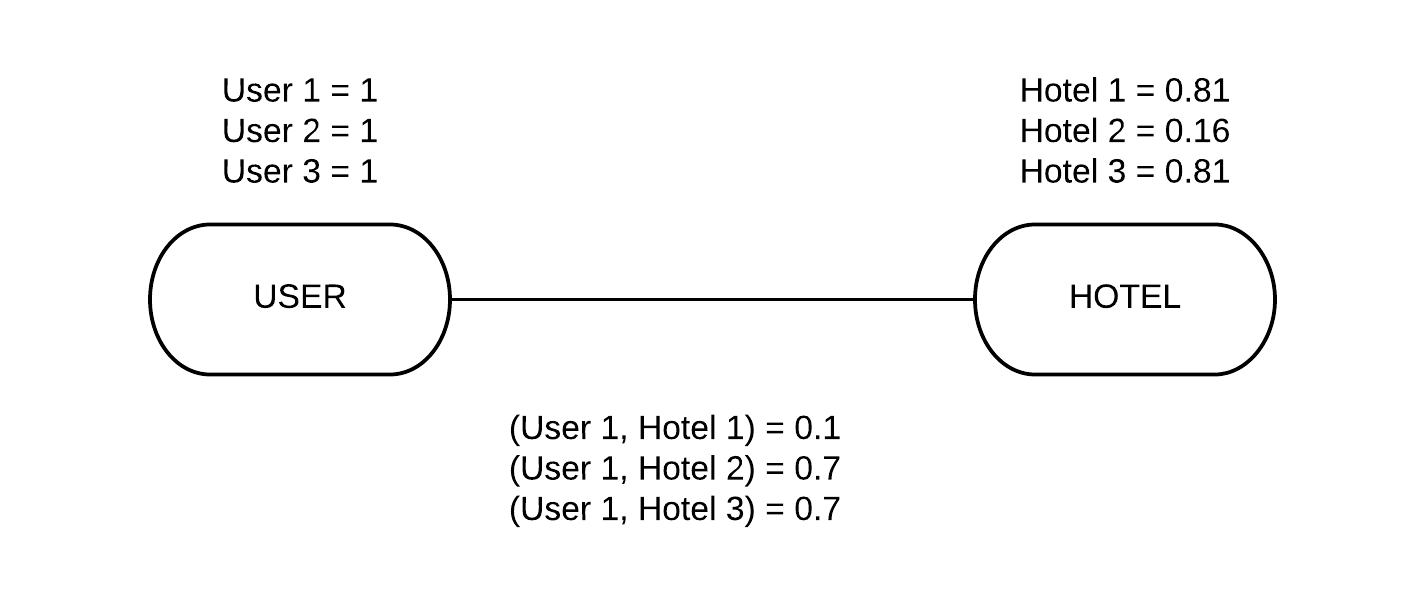
\includegraphics{images/softcsp-bw.png}
		\caption{Esempio con vincoli soft}
	\end{figure}
	
	Quindi effettuando la combinazione dei valori i risultati sono:
	
	\$(User1 , Hotel 1) = 1 + 0.1 + 0.81 = 1.91\$
	
	\$(User 1, Hotel 2) = 1 + 0.7 + 0.16 = 1.86\$
	
	\$(User 1, Hotel 3) = 1 + 0.7 + 0.81 = 2.51\$
	
	Giunti a questo punto si utilizza l'operatore di ottimizzazione per
	ottenere il risultato ossia l'\emph{operatore di massimo} (max) ed il
	risultato ottenuto è la combinazione \emph{User 1 \& Hotel 3}. Che di
	fatto rappresenta la migliore scelta per l'utente 1.
	
	\hypertarget{header-n280}{%
		\subsection{Conclusioni}\label{header-n280}}
	
	A differenza dell'algoritmo di CasMin individuato da Josang la nostra
	soluzione per scegliere l'elemento di preferenza migliore non da
	priorità alle preferenze che hanno un voto ``medio/alto" per entrambi i
	sistemi (quello di reputazione e quello di raccomandazione) ma bensì
	ottimizza il soddisfacimento in generale. Quindi in molti casi la
	soluzione proposta dallo studio di Josang e la nostra riportano i
	medesimi risultati ma potrebbero esserci casi in cui questo non è
	verificato. Suggeriamo di consultare la sezione riguardo alla nostra
	implementazione per avere ulteriori riscontri.
	
	\hypertarget{header-n284}{%
		\section{La nostra implementazione}\label{header-n284}}
	
	\hypertarget{header-n287}{%
		\section{Bibliografia}\label{header-n287}}
	
	\begin{enumerate}
		\item
		\href{https://www.researchgate.net/publication/262187804_Combining_Recommender_and_Reputation_Systems_to_Produce_Better_Online_Advice}{\textit{Combining Recommender and Reputation Systems to Produce Better Online Advice}}, Audun Jøsang, Guibing Guo, Maria Silvia Pini, Francesco Santini, Yue Xu
		\item \href{https://www.sciencedirect.com/science/article/pii/S1110866515000341}{\textit{Recommendation systems: Principles, methods and evaluation}}, F.O.Isinkaye Y.O.Folajimi B.A.Ojokoh
		\item 
		\href{https://link.springer.com/article/10.1007/s12599-017-0493-1}{\textit{Interactive Reputation Systems}}, Johannes Sänger Günther Pernul
	\end{enumerate}
	
\end{document}